This page is organized as follows\+:
\begin{DoxyItemize}
\item \hyperlink{src_HLS_page_HLS_overview}{High-\/\+Level Synthesis overview} presents the general outlines of the high-\/level synthesis problem.
\item \hyperlink{src_HLS_page_HLS_problem}{Problem description} defines the problem in a formal way.
\item \hyperlink{src_HLS_page_HLS_bambu}{Datastructure in the Bambu tool} describes how informations are stored in the Bambu tool and how they can be retrieved.
\end{DoxyItemize}\hypertarget{src_HLS_page_HLS_overview}{}\section{High-\/\+Level Synthesis overview}\label{src_HLS_page_HLS_overview}
Forty years ago, Electronics Magazine asked Intel co-\/founder Gordon Moore to write an article summarizing the state of the electronics industry. When writing the article, Moore noted that the number of devices (which then included transistors and resistors) inside chips was doubling every year, largely because engineers could shrink the size of transistors. That meant that the performance and capabilities of semiconductors were growing exponentially and would continue to. In 1975, Moore amended the law to state that the number of transistors doubled about every 24 months.

Very-\/large-\/scale integration (V\+L\+SI) is the process of creating integrated circuits (IC) by combining thousands of transistor-\/based circuits into a single chip. V\+L\+SI began in the 1970s when complex semiconductor and communication technologies were being developed. Modern I\+Cs are enormously complicated. A large chip may well have more transistors than people on Earth within few years\+: V\+L\+SI technology provides densities of multiple-\/million gates of logic per chip. Furthermore, the rules for what can and cannot be manufactured are also extremely complex. An integrated circuit process as of 2006 may well have more than 600 rules.

Chip of such complexity are very difficult, if not impossible, to design using the traditional {\itshape capture-\/and-\/simulate} design methodology. Instead, time to market is usually equally, if not more important than area or speed. So the industry has started looking at the product development cycle comprehensively to reduce the design time and to gain a competitive edge in the time-\/to-\/market race.

As the complexity of chips increases, so will the need for design automation on higher level of abstraction, where functionality is easier to understand and trade-\/off is more influential. There are several advantages to automating part or all of the design process and moving automation to higher levels. First, automation assures a much shorter design cycle. Then, it allows for more exploration at different design styles since different designs can be generated and evaluated quickly. Finally, design automation tools may out-\/perform average human designers in meeting most design constraints and requirements.

{\bfseries Computer-\/aided tools} provide an effective mean for designing microelectronic circuits that are economically viable products. Synthesis techniques speed up the design cycle and reduce the human effort. Optimization techniques enhance the design quality. At present, synthesis and optimization techniques are used for most digital circuit designs. Nevertheless their power is not yet exploited in full and most of the work is still made by hand.\hypertarget{src_HLS_page_sec_synthesis}{}\subsection{The synthesis process}\label{src_HLS_page_sec_synthesis}
{\itshape {\bfseries Synthesis}} is the generation of a circuit model, starting from a less detailed one. Models can be classified in terms of levels of abstraction and views. We consider here three main abstractions, namely\+: {\itshape architectural}, {\itshape logic} and {\itshape geometrical}. The levels can he visualized as follows. At the {\itshape architectural level} a circuit performs a set of operations, such as data computation or transfer. At the {\itshape logic level}, a digital circuit evaluates a set of logic functions. At the {\itshape geometrical level}, a circuit is a set of geometrical entities.

The architectural-\/level synthesis consists of generating a structural view of an architectural-\/level model. This corresponds to determining an assignment of the circuit functions to operators, called resources, as well as their interconnection and the timing of their execution. It has also been called {\bfseries high-\/level synthesis} or {\bfseries structural synthesis}, because it determines the macroscopic (i.\+e., block-\/level) structure of the circuit. A behavioral architectural-\/level model can be abstracted as a set of operations and dependencies. Architectural synthesis entails identifying the hardware resources that can implement the operations, scheduling the execution time of the operations and binding them to the resources. In other words, synthesis defines a structural model of a data path, as an interconnection of resources, and a logic-\/level model of a control unit, that issues the control signals to the data path according to the schedule. After the architectural-\/level synthesis, the {\itshape logic-\/level synthesis} step has to be performed. Logic-\/level synthesis is the task of generating a structural view of a logic-\/level model. Logic synthesis is the manipulation of logic specifications to create logic models as an interconnection of logic primitives. Thus logic synthesis determines the microscopic (i.\+e., gate-\/level) structure of a circuit. The task of transforming a logic model into an interconnection of instances of library cells, i.\+e., the back end of logic synthesis, is often referred to as library binding or technology mapping. A logic-\/level model of a circuit can be provided by a state transition diagram of a finite-\/state machine, by a circuit schematic or equivalently by an H\+DL model. It may be specified by a designer or synthesized from an architectural-\/level model. The logic synthesis tasks may be different according to the nature of the circuit (e.\+g., sequential or combinational) and to the initial representation (e.\+g., state diagram or schematic). Since many are the possible configurations of a circuit, optimization plays a major role, in connection with synthesis, in determining the microscopic figures of merit of the implementation. The final outcome of logic synthesis is a fully structural representation, such as a gate-\/level netlist. The final step is the {\itshape geometrical-\/level synthesis}, that consists of creating a physical view at the geometric level. It entails the specification of all geometric patterns defining the physical layout of the chip, as well as their position. It is often called physical design, and we shall call it so. Physical design consists of generating the layout of the chip. The layers of the layout are in correspondence with the masks used for chip fabrication. Therefore, the geometrical layout is the final target of microelectronic circuit design. Physical design depends much on the design style. On one end of the spectrum, for custom design, physical design is handcrafted by using layout editors. This means that the designer renounces the use of automated synthesis tools in the search for optimizing the circuit geometries by fine hand-\/tuning. On the opposite end of the spectrum, in case of prewired circuits, physical design is performed in a virtual fashion, because chips are fully manufactured in advance. The major tasks in physical design are placement and wiring, called also routing. Cell generation is essential in the particular case of macro-\/cell design, where cells are synthesized and not extracted from a library.

Logic-\/level and physic synthesis steps have already been consistently automatized; for instance, logic synthesis has been well performed by Altera and Xilinx in their synthesis tools for F\+P\+GA design. The main problem up to now is that these tools require a R\+TL design described through an hardware description language to be synthesized. So a further step into design automation is to develop tools able to bridge the gap between behavioral specification and R\+TL design. This kind of tools have to be able to produce R\+TL design in a quite short time, with respect to design constraints. Besides, they have to be able to explore larger and larger design space region to find better and better solutions with respect to design goals. This is why {\itshape high-\/level synthesis} has been a very hot research topic over past two decades.\hypertarget{src_HLS_page_HLS_problem}{}\section{Problem description}\label{src_HLS_page_HLS_problem}
{\itshape High-\/\+Level Synthesis} (H\+LS) is defined as a translation process from behavioural description into register-\/transfer-\/level (R\+TL) structural description. It can be considered the automation of first step of the design flow, the architectural-\/level synthesis.

The inputs to a typical H\+LS tool include a {\itshape behavioral description}, a {\itshape resource library} describing available hardware resources and a set of {\itshape design constraints}.

The output from a high-\/level synthesizer consists of two parts\+: a datapath structure at the register-\/transfer level (R\+TL) and a specification of the finite state machine to control the datapath. At the R\+TL level, a datapath is composed of functional units, storage and interconnection elements. The finite state machine specifies every set of microoperations for the datapath to be performed during each control step. The output can be then synthesized using related tools.

The goal is to reduce one or more design targets. Objectives can be to minimize total area occupied, latency or power consumption.

{\itshape Behavioral description} specifies behaviour in terms of operations, assignment statements, and control constructs in a common high-\/level language (e.\+g. C language). In the Bambu tool, it is represented by the class behavioral\+\_\+manager.

In the {\itshape resource library}, there may be several alternatives among which the synthesizer must select the one that best matches the design constraints and maximizes the optimization objective. In the Bambu tool, it is represented by the class \hyperlink{classtechnology__manager}{technology\+\_\+manager}.

The {\itshape constraints} can be on the maximum number of available units of each resources, on total area or on the latency of the specification execution. In the Bambu tool, it is represented by the class \hyperlink{classHLS__constraints}{H\+L\+S\+\_\+constraints}.

There are two main tasks in high-\/level synthesis\+: operations scheduling and resources allocation. {\itshape \hyperlink{classScheduling}{Scheduling}} provides the control steps in which operations start their execution (see \hyperlink{src_HLS_scheduling_general}{Scheduling}). {\itshape Resource allocation} (see \hyperlink{src_HLS_allocation_page}{Allocation} and \hyperlink{src_HLS_binding_page}{Binding}) is concerned with assigning operations and values to hardware components and interconnect them using connection elements. Solving these problems efficiently is a non-\/trivial matter because of their N\+P-\/complete nature. Furthermore, the objectives are usually in contrast and the best high-\/level synthesis design flow cannot be known a priori since it depends heavily on nature of the problem\+: on some examples, executing scheduling before allocation can leads to better results, on other examples, it can leads to worse ones.

The remaining task is the creation of the structural representation of the datapath and the controller units (see \hyperlink{src_HLS_datapath_page}{Datapath creation} and \hyperlink{src_HLS_controller_fsm}{Controller Synthesis}).\hypertarget{src_HLS_page_HLS_bambu}{}\section{Datastructure in the Bambu tool}\label{src_HLS_page_HLS_bambu}
"\hyperlink{classScheduling}{Scheduling} assigns operations in the behavioral description to control steps. Within each control step, a separate functional unit is required to execute each operation assigned to that step.

After scheduling, the datapath is constructed in two steps\+: unit allocation and unit binding; some researchers call unit allocation and unit binding collectively as datapath allocation. Unit allocation determines the number and types of RT components to be used in the design. Since a real RT component library may contain multiple types of functional units, each with different characteristics (e.\+g., functionality, size, delay and power dissipation), unit allocation needs to determine the number and types of different functional and storage units present in the component library. Unit binding maps the operations, variables, and data transfers from the scheduled C\+D\+FG to the functional, storage and interconnection units, respectively, while ensuring that the design behavior operates correctly on the selected set of components. Unit binding consists of three interdependent tasks\+: storage binding, functional-\/unit binding, and interconnection binding. Storage binding maps data carriers (e.\+g., constants, variables and data structures like arrays) in the behavioral description onto storage elements (e.\+g., R\+O\+Ms, registers and memory units) in the datapath. Functional-\/unit binding involves the mapping of operations in the behavioral description to the set of selected functional units. Interconnection binding maps every data transfer in the behavior into a set of interconnection units for data routing"\mbox{[}1\mbox{]}.\hypertarget{src_HLS_page_src_HLS_phases}{}\section{Phases}\label{src_HLS_page_src_HLS_phases}

\begin{DoxyItemize}
\item Subproject \hyperlink{src_HLS_scheduling_general}{Scheduling} provides scheduling algorithms.
\item Subproject \hyperlink{src_HLS_allocation_page}{Allocation} provides facilities for functional unit allocation
\item Subproject \hyperlink{src_HLS_binding_constraints_page}{Binding constraints} provides facilities for operation binding on functional units
\item Subproject \hyperlink{src_HLS_binding_page}{Binding} provides synthesis algorithms about register allocation, module binding optimization and interconnetion allocation.
\item Subproject \hyperlink{src_HLS_datapath_page}{Datapath creation} creates structural representation about datapath
\item Subproject \hyperlink{src_HLS_controller_fsm}{Controller Synthesis} creates structural representation about controller
\item Subproject src\+\_\+\+H\+L\+S\+\_\+hls\+\_\+flow\+\_\+page contains implemented high-\/level synthesis flow
\end{DoxyItemize}\hypertarget{src_HLS_page_src_HLS_additional}{}\section{Additional subprojects}\label{src_HLS_page_src_HLS_additional}

\begin{DoxyItemize}
\item Subproject \hyperlink{src_HLS_estimation}{High-\/level syntesis result estimation} provides some metrics for result estimation
\end{DoxyItemize}\hypertarget{src_HLS_page_src_HLS_data_structure}{}\section{Data structures}\label{src_HLS_page_src_HLS_data_structure}
This section describes the data structures used in High Level Synthesis algorithm. Typically a High Level Synthesis task is divided in four stages and our algorithm follows this division\+:
\begin{DoxyItemize}
\item \hyperlink{classScheduling}{Scheduling} and functional unit binding;
\item Register Binding;
\item Interconnection Binding;
\item Datapath and Controller generation. ~\newline
 For each of this stages a set of variables are defined in class hls. For scheduling problem the variable to be used are\+:
\item sch;
\item fu. ~\newline
 For register binding the variables are\+:
\item bind;
\item bind\+\_\+const. ~\newline
 For interconnection binding and datapath (controller) creation the variables are\+:
\item Datapath;
\item Fsm. ~\newline
 These structures will described more in detail in the next sections. 
\end{DoxyItemize}\hypertarget{src_HLS_page_src_HLS_data_structure_scheduling}{}\subsection{Scheduling data structures}\label{src_HLS_page_src_HLS_data_structure_scheduling}
The hls struct contains some variables that are used to represent an intermediate layer for all scheduling algorithm. These variables are sch and fu. \hypertarget{src_HLS_page_sch}{}\subsubsection{sch}\label{src_HLS_page_sch}
It is used to map operations on control steps; this variable is built during the execution of the scheduling algorithm. They type of this variable is {\itshape sdt\+::map$<$vertex, unsigned int$>$}\+: each vertex has associated the control step in which the operation (represented by the vertex itself) is executed. \hypertarget{src_HLS_page_fu}{}\subsubsection{fu}\label{src_HLS_page_fu}
This variable stores, for all scheduled operations, where they are executed. This structure is composed of two element\+: one (the first), named \char`\"{}assign\char`\"{}, stores the type of the functional unit that has to perform the specific operation; the other, named \char`\"{}index\char`\"{}, stores the instance of functional unit (identified by assign) that has to perform the operation. \hypertarget{src_HLS_page_src_HLS_data_structure_binding}{}\subsection{Register binding data structures}\label{src_HLS_page_src_HLS_data_structure_binding}
There are four structures used by the register binding problem\+: bind, bind\+\_\+const, used\+\_\+reg and used\+\_\+const. These structures must be used by all register binding algorithms as an intermediate layer. \hypertarget{src_HLS_page_bind}{}\subsubsection{bind}\label{src_HLS_page_bind}
This variable maps all values in the system specification to a register. This variable is used by all register binding algorithms. The type of this variable is {\itshape std\+::map $<$ std\+::pair$<$vertex , unsigned int$>$ , int $>$}\+: the first field represents the value to be stored, and it is a pair operation variable; the second is an integer number which represents the specific instance of the register used to store the value. \hypertarget{src_HLS_page_bind_const}{}\subsubsection{bind\+\_\+const}\label{src_HLS_page_bind_const}
This variable maps the constants, specified in the system, on the storage units. This variable must be used to create a working datapath. Because the binding of the constants is not required in register binding algorithm, is not required that this variable has to be used from binding algorithms. The structure of this variable is equal to the structure of variable bind. \hypertarget{src_HLS_page_used_reg}{}\subsubsection{used\+\_\+reg}\label{src_HLS_page_used_reg}
This variable stores the number of register used. \hypertarget{src_HLS_page_used_const}{}\subsubsection{used\+\_\+const}\label{src_HLS_page_used_const}
This variable stores the number of constants used. \hypertarget{src_HLS_page_src_HLS_data_structure_datapath}{}\subsection{Interconnection binding data structures}\label{src_HLS_page_src_HLS_data_structure_datapath}
\hypertarget{src_HLS_page_datapath}{}\subsubsection{datapath}\label{src_HLS_page_datapath}
Data structure storing the structural description of the datapath, in term of\+:
\begin{DoxyItemize}
\item component (even with gerarchic structure);
\item channel (even with gerarchic structure);
\item signal;
\item input, output and generic port;
\item interface. This representation has to be created after the application of an interconnection binding algorithm, to complete the datapath description, after the scheduling (with fu binding) and register binding phases. 
\end{DoxyItemize}\hypertarget{src_HLS_page_src_HLS_data_structure_fsm}{}\subsection{Controller creation}\label{src_HLS_page_src_HLS_data_structure_fsm}
\hypertarget{src_HLS_page_FSM}{}\subsubsection{F\+SM}\label{src_HLS_page_FSM}
The {\bfseries F\+SM} variable stores a pointer to the circuit implementing the architecture of the controller. This field must be filled after the datapath creation. There are some support variables, which will be introduced in the next sections, which contain informations usefull for the controller creation. \hypertarget{src_HLS_page_src_HLS_data_structure_other}{}\subsection{Other data structure}\label{src_HLS_page_src_HLS_data_structure_other}
This section introduces some usefull variables, which must be used to couple the controller with the datapath. \hypertarget{src_HLS_page_input_enable_port}{}\subsubsection{input\+\_\+enable\+\_\+port}\label{src_HLS_page_input_enable_port}
This variable is managed by datapath (interconnection binding) and fsm creation algorithms; its type is {\itshape std\+::map$<$ vertex , std\+::set$<$ int $>$ $>$}\+: each vertex (i.\+e. operation) has associated a set of integers, which are index in the \char`\"{}in\+\_\+port\+\_\+map\char`\"{} variable, described below. The datapath creation part fills this data structure with the reference to the input ports that have to be set to true to perform the memorization of a value in a register when each operation (as I\textquotesingle{}ve just said operations and vertex are used here as synonims) is executed. The F\+SM creation algorithm must visit this structure and, according with the result of the scheduling phase, it nust set the approriate port in the \char`\"{}in\+\_\+port\+\_\+map\char`\"{} field associated with the integer contained in input\+\_\+enable\+\_\+port \hypertarget{src_HLS_page_input_address_port}{}\subsubsection{input\+\_\+address\+\_\+port}\label{src_HLS_page_input_address_port}
This variable is managed by datapath (interconnection binding) and fsm creation algorithms; its type is {\itshape std\+::map$<$ vertex , std\+::set$<$ std\+::pari$<$int, int$>$ $>$ $>$}\+: each vertex (i.\+e. operation) has a pair associated\+: the first element is an index in the \char`\"{}in\+\_\+port\+\_\+map\char`\"{} variable, described below, the second element the value which must be asserted on the associated port (the association is contained in the \char`\"{}in\+\_\+port\+\_\+map\char`\"{} variable), in order to perform the selection of mux input (or the enable of tristate). The datapath creation part fills this data structure with the reference to the input ports that have to be set to true to perform the memorization of a value in a register when each operation (as I\textquotesingle{}ve just said operations and vertex are used here as synonims) is executed. The F\+SM creation algorithm has to visit this structure and, according with the result of the scheduling phase, sets the value to the appropriated ports. This variable is composed of two fields. The first represents the operations, the second is a pair formed by an index in the \char`\"{}in\+\_\+port\+\_\+map\char`\"{} variable which points to the address port which must be set when the specified operation is performed, and the 32 bit integer value which must be issued on that port. This variable considers also tristate enables, because this enables has to be setted at the beginning of a control step, while the register enables have to be setted at the end of the control step. A convention is introduced about the value to set. If the value is greater or equal to zero, this value represents a mux address, otherwise, if the value is equal to \char`\"{}-\/1\char`\"{}, it represents a tristate enable. \hypertarget{src_HLS_page_output_port}{}\subsubsection{output\+\_\+port}\label{src_HLS_page_output_port}
This variable, whose type is again {\itshape std\+::map $<$ vertex , int $>$} stores the association between the conditional output ports of the datapath and and index in the \char`\"{}out\+\_\+port\+\_\+map\char`\"{}, which in turn has associated the id of the input port in the controller. With conditional output ports I mean the ports which carry the result of conditional operations (if, while...) so just conditional vertex should have an entry in this field. \hypertarget{src_HLS_page_in_port_map}{}\subsubsection{in\+\_\+port\+\_\+map}\label{src_HLS_page_in_port_map}
This variable is filled during the controller creation step\+: it is again a map and it associates an index in the \char`\"{}input\+\_\+address\+\_\+port\char`\"{} or \char`\"{}input\+\_\+enable\+\_\+port\char`\"{} variables with the index of the desired port in the fsm circuit. \hypertarget{src_HLS_page_out_port_map}{}\subsubsection{out\+\_\+port\+\_\+map}\label{src_HLS_page_out_port_map}
This variable is filled during the controller creation step\+: it is again a map and it associates an index in the \char`\"{}output\+\_\+port\char`\"{} variable with the index of the desired port in the fsm circuit. \hypertarget{src_HLS_page_bind_write_port}{}\subsubsection{bind\+\_\+write\+\_\+port}\label{src_HLS_page_bind_write_port}
This variable has to be managed by the datapath creation algorithms. The algorithm, during datapath creation, maps the vertex that write an output on the relative output port. \hypertarget{src_HLS_page_convertion_map}{}\subsubsection{convertion\+\_\+map}\label{src_HLS_page_convertion_map}
This variable maps all the input and output data port of the system with the relative variable. During datapath creation this variable is filled, as shown in the next example. \hypertarget{src_HLS_page_src_HLS_data_strucutre_example}{}\subsection{Example}\label{src_HLS_page_src_HLS_data_strucutre_example}
This section provides a simple example of the hls flow. Lets start with the specification of the problem; suppose to have the following specification\+:~\newline
~\newline
 +1 \+: a = i1 + c1 ;~\newline
 -\/1 \+: b = i2 -\/ c1 ;~\newline
 +2 \+: o1 = a + b ;~\newline
~\newline
 The most relevant graphs that will be created are\+:
\begin{DoxyItemize}
\item F\+S\+DG; 
\begin{DoxyImageNoCaption}
  \mbox{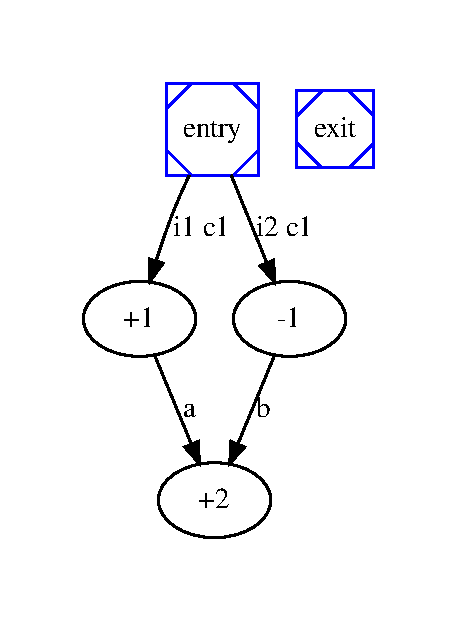
\includegraphics[width=\textwidth,height=\textheight/2,keepaspectratio=true]{dot_inline_dotgraph_22}}
\end{DoxyImageNoCaption}

\item BB; 
\begin{DoxyImageNoCaption}
  \mbox{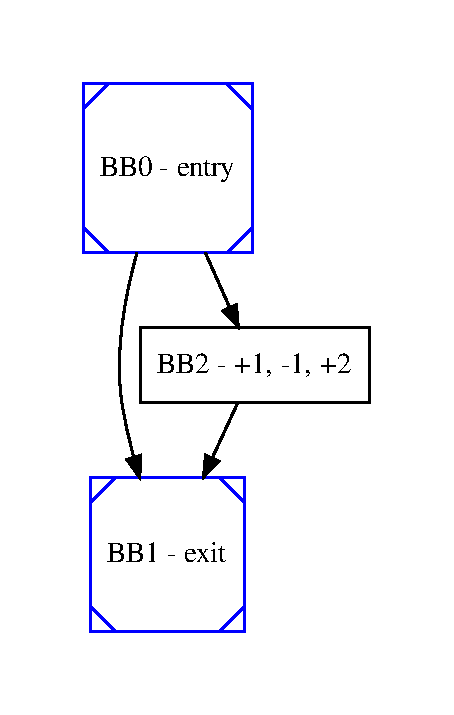
\includegraphics[width=\textwidth,height=\textheight/2,keepaspectratio=true]{dot_inline_dotgraph_23}}
\end{DoxyImageNoCaption}
 
\end{DoxyItemize}\hypertarget{src_HLS_page_Scheduling}{}\subsubsection{Scheduling}\label{src_HLS_page_Scheduling}
Suppose to have 1 plus and 1 minus functional unit. During the scheduling phase these information are written\+:
\begin{DoxyItemize}
\item variable sch ~\newline
 +1 =$>$ control step 0;~\newline
 -\/1 =$>$ control step 0;~\newline
 +2 =$>$ control step 1;~\newline

\item variable \hyperlink{classfu__binding}{fu\+\_\+binding} ~\newline
 +1 =$>$ $<$plus,0$>$;~\newline
 -\/1 =$>$ $<$minus,0$>$;~\newline
 +2 =$>$ $<$plus,0$>$;~\newline

\end{DoxyItemize}\hypertarget{src_HLS_page_Binding}{}\subsubsection{Binding}\label{src_HLS_page_Binding}
The data which is produced in this step is\+:
\begin{DoxyItemize}
\item variable bind ~\newline
 $<$ +1 , a $>$ =$>$ register 0;~\newline
 $<$ -\/1 , b $>$ =$>$ register 1;~\newline

\item variable used\+\_\+regis~\newline
 used\+\_\+regis = 2;~\newline

\item variable bind\+\_\+const ~\newline
 $<$ Entry , c1 $>$ =$>$ constant storage 0;~\newline

\item variable used\+\_\+const~\newline
 used\+\_\+const = 1;~\newline

\item variable bind\+\_\+write\+\_\+port ~\newline
 $<$ +2 , o1 $>$ =$>$ W\+R\+I\+T\+E\+\_\+\+P\+O\+RT 0; 
\end{DoxyItemize}\hypertarget{src_HLS_page_Datapath}{}\subsubsection{Datapath}\label{src_HLS_page_Datapath}
Now the datapath of the circuit can be created. First of all we must perform the connection binding\+: this operation is executed with several operation and can use several data structure that are not presented here. In this section will only show the datapath, and the intermediate structure used to support the controller creation. A simplified view of the datapath is 
\begin{DoxyImageNoCaption}
  \mbox{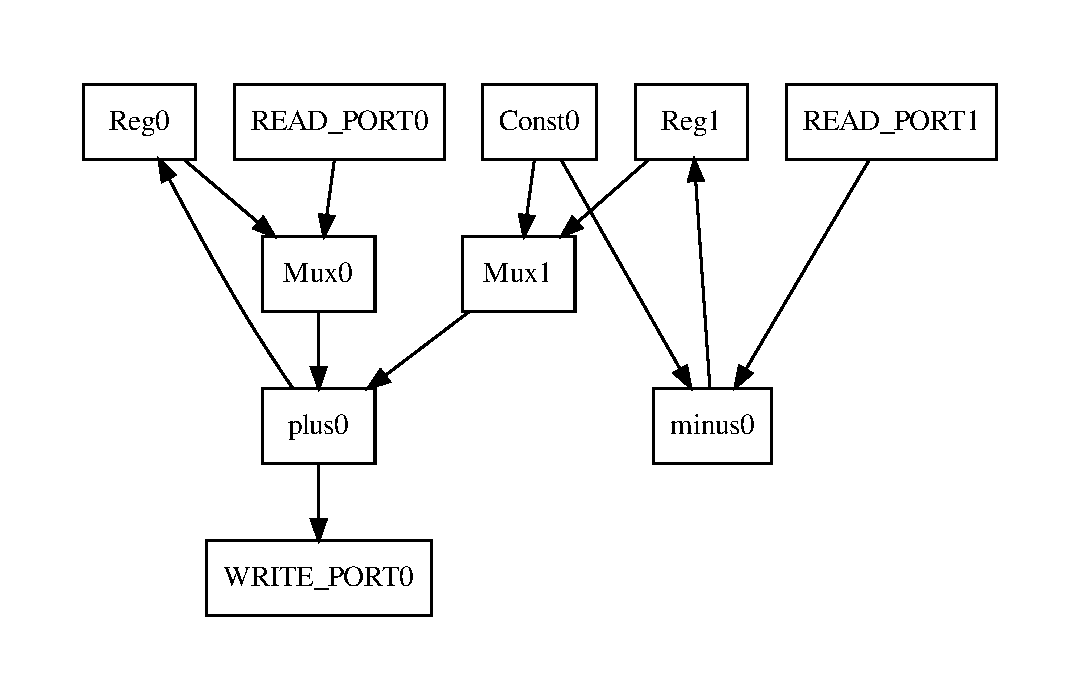
\includegraphics[width=\textwidth,height=\textheight/2,keepaspectratio=true]{dot_inline_dotgraph_24}}
\end{DoxyImageNoCaption}
 The support data structure are\+:
\begin{DoxyItemize}
\item input\+\_\+address\+\_\+port (Mux$\ast$\+\_\+ra represent the integer reference to datapath port, i.\+e. the index in the in\+\_\+port\+\_\+map field) ~\newline
 +1 =$>$ $<$ Mux0\+\_\+ra , 0 $>$ , $<$ Mux1\+\_\+ra , 0 $>$ ;~\newline
 -\/1 =$>$ ;~\newline
 +2 =$>$ $<$ Mux0\+\_\+ra , 1 $>$ , $<$ Mux1\+\_\+ra , 1 $>$ ;~\newline

\item input\+\_\+enable\+\_\+port (Reg$\ast$\+\_\+re represent the integer reference to datapath port) ~\newline
 +1 =$>$ $<$ Reg0\+\_\+re $>$ ; ~\newline
 -\/1 =$>$ $<$ Reg1\+\_\+re $>$ ; ~\newline
 +2 =$>$ ; ~\newline

\item output\+\_\+port ~\newline
 For this example is empty\+: there are no conditional (if, while, switch...) vertex.~\newline

\item convertion\+\_\+map~\newline
 R\+E\+A\+D\+\_\+\+P\+O\+R\+T0 =$>$ i1;~\newline
 R\+E\+A\+D\+\_\+\+P\+O\+R\+T1 =$>$ i2;~\newline
 W\+R\+I\+T\+E\+\_\+\+P\+O\+R\+T0 =$>$ o1;~\newline
 
\end{DoxyItemize}\hypertarget{src_HLS_page_Controller}{}\subsubsection{Controller}\label{src_HLS_page_Controller}
Previously described data structures are used for the generation of the controller, too. In particular, the S\+DG is analysed to build a finite state machine in which all data and control constraints are respected. There are two types of F\+SM output, which correspond to the two types of datapath input\+: enabling signals (1 bit), and addresses (currently 32 bit). ~\newline
H\+LS data structures input\+\_\+address\+\_\+port and input\+\_\+enable\+\_\+port are used in F\+SM generation to produce the right output at the right control step. ~\newline
Continuing the example above\+:~\newline

\begin{DoxyItemize}
\item input\+\_\+address\+\_\+port ~\newline
+1 =$>$ $<$ Mux0\+\_\+ra , 0 $>$ , $<$ Mux1\+\_\+ra , 0 $>$ means that the ports indexed by Mux0\+\_\+ra and Mux1\+\_\+ra must be set to 0 at the F\+SM state associated by the schedule to operation +1; ~\newline
Operation -\/1 has no entry because there is no need to set any address when executing it;~\newline
+2 =$>$ $<$ Mux0\+\_\+ra , 1 $>$ , $<$ Mux1\+\_\+ra , 1 $>$ means that the ports indexed by Mux0\+\_\+ra and Mux1\+\_\+ra must be set to 1 at the F\+SM state associated by the schedule to operation +2; ~\newline

\item input\+\_\+enable\+\_\+port ~\newline
+1 =$>$ $<$ Reg0\+\_\+re $>$ means that the port indexed by Reg0\+\_\+re must be set H\+I\+GH at the F\+SM state associated by the schedule to operation +1; ~\newline
-\/1 =$>$ $<$ Reg1\+\_\+re $>$ means that the port indexed by Reg1\+\_\+re must be set H\+I\+GH at the F\+SM state associated by the schedule to operation -\/1; ~\newline
+2 has no entry beacuse no enabling signal must be set H\+I\+GH for the execution of operation +2;~\newline
Notice that output unspecified in the input\+\_\+enable\+\_\+port data structure must be set L\+OW in all the other F\+SM state, while unspecified addresses can be set to any other value, either left unchanged or set to some conventional value for further optimization possibly performed by synthesis tools.~\newline

\item in\+\_\+port\+\_\+map is filled by the F\+SM generator algorithm to associate a circuit port with the indexes specified in the \char`\"{}input\+\_\+address\+\_\+port\char`\"{} or \char`\"{}input\+\_\+enable\+\_\+port\char`\"{} variables. ~\newline
In the example above (Mux$\ast$\+\_\+ra and Reg$\ast$\+\_\+re represent the integer reference to datapath input port (and also the index in the in\+\_\+port\+\_\+map structure), while F\+S\+M\+Mux$\ast$\+\_\+ra and F\+S\+M\+Reg$\ast$\+\_\+re represet the integer reference to associated output port in the F\+SM circuit)\+: ~\newline
$<$ Reg0\+\_\+re, F\+S\+M\+Reg0\+\_\+re $>$~\newline
$<$ Reg1\+\_\+re, F\+S\+M\+Reg1\+\_\+re $>$~\newline
$<$ Mux0\+\_\+ra, F\+S\+M\+Mux0\+\_\+ra $>$~\newline

\item out\+\_\+port\+\_\+map ~\newline
For this example is empty\+: there are no conditional (if, while, switch...) vertex.~\newline
 
\end{DoxyItemize}\hypertarget{src_HLS_page_References}{}\section{References}\label{src_HLS_page_References}
\mbox{[}1\mbox{]} Recent Development in High Level Synthesisy Youn-\/\+Long Lin Department of Computer Science Tsing Hua University Hsin-\/\+Chu, Taiwan 30043, R. O. C. 